% =====================================================================
%  Front cover — The Shape of the Threat
%  Typeset standalone at the 6 x 9 in trim, full bleed.
%  Vertical positions are in inches measured from the foot of the page.
% =====================================================================
\documentclass{article}
\usepackage[paperwidth=6in,paperheight=9in,margin=0pt]{geometry}
\usepackage{fontspec}
\usepackage{xcolor}
\usepackage{graphicx}
\usepackage{tikz}

\setmainfont{Outfit}[
  UprightFont={Outfit Regular}, BoldFont={Outfit Bold},
  ItalicFont={Outfit Regular}, ItalicFeatures={FakeSlant=0.20},
  BoldItalicFont={Outfit Bold}, BoldItalicFeatures={FakeSlant=0.20},
  Ligatures={TeX}]
% The cover sets most of its type in \sffamily. Without an explicit
% sans face that is Latin Modern Sans, so the cover would carry two
% typefaces where the book carries one.
\setsansfont{Outfit}[
  UprightFont={Outfit Regular}, BoldFont={Outfit Bold},
  ItalicFont={Outfit Regular}, ItalicFeatures={FakeSlant=0.20},
  BoldItalicFont={Outfit Bold}, BoldItalicFeatures={FakeSlant=0.20},
  Ligatures={TeX}]
\setmonofont{DejaVu Sans Mono}[
  UprightFont={DejaVu Sans Mono}, BoldFont={DejaVu Sans Mono Bold},
  Ligatures={TeX}]

\definecolor{ink}{HTML}{080B14}
\definecolor{accent}{HTML}{E8B85C}
\definecolor{txt}{HTML}{E6E9F0}
\definecolor{dim}{HTML}{939BAB}

\pagestyle{empty}
\setlength{\parindent}{0pt}

\begin{document}
\begin{tikzpicture}[remember picture,overlay]
  % ---- the plate, full bleed --------------------------------------------
  \node[anchor=south west,inner sep=0] at (current page.south west)
    {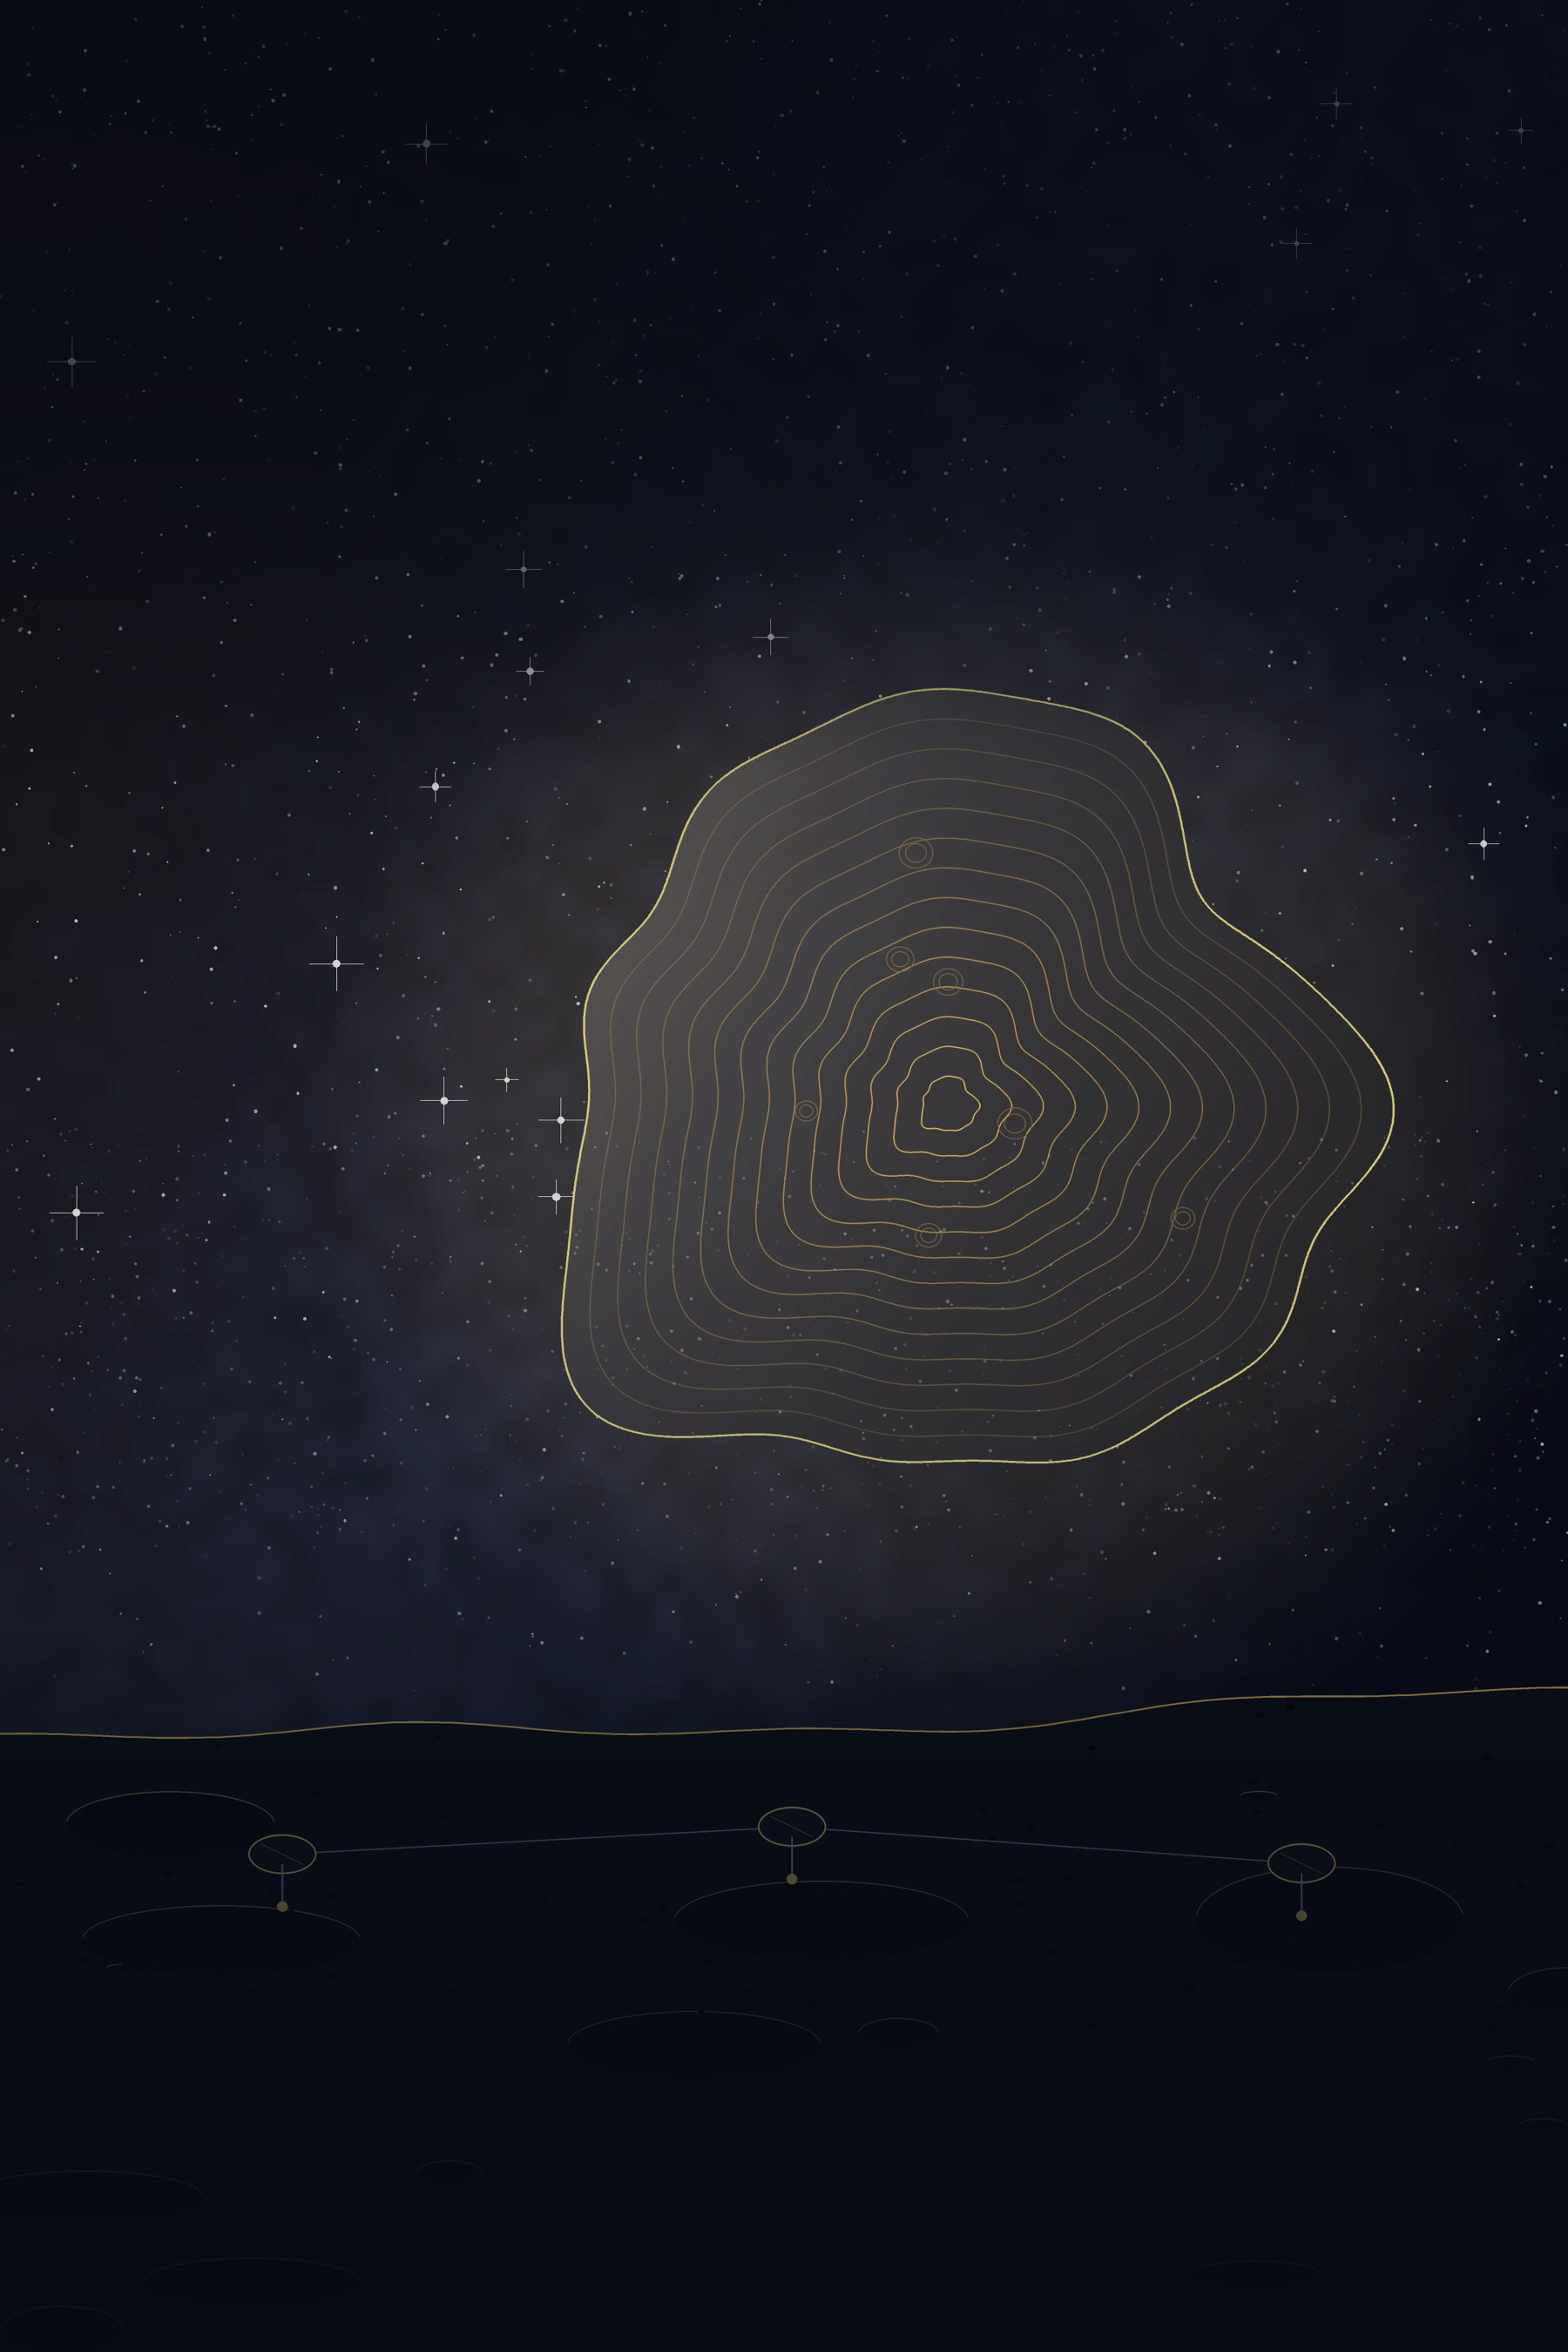
\includegraphics[width=\paperwidth,height=\paperheight]{../figures/cover_front_art.jpg}};

  % ---- identity block ----------------------------------------------------
  \node[anchor=south west,inner sep=0,text=accent] at ([xshift=0.60in,yshift=8.50in]current page.south west)
    {\fontsize{6.8}{8.2}\selectfont\sffamily
     \addfontfeatures{LetterSpace=16}A CASE FOR ACCOUNTABILITY IN PLANETARY DEFENCE};

  \fill[accent] ([xshift=0.60in,yshift=8.32in]current page.south west)
         rectangle ([xshift=5.40in,yshift=8.345in]current page.south west);

  \node[anchor=south west,inner sep=0,text=txt] at ([xshift=0.60in,yshift=7.84in]current page.south west)
    {\fontsize{42}{46}\selectfont\sffamily\bfseries THE SHAPE};

  \node[anchor=south west,inner sep=0,text=txt] at ([xshift=0.60in,yshift=7.24in]current page.south west)
    {\fontsize{42}{46}\selectfont\sffamily\bfseries OF THE THREAT};

  \fill[accent] ([xshift=0.60in,yshift=7.02in]current page.south west)
         rectangle ([xshift=5.40in,yshift=7.045in]current page.south west);

  \node[anchor=south west,inner sep=0,text=dim,align=left] at ([xshift=0.60in,yshift=6.58in]current page.south west)
    {\fontsize{10.4}{13.4}\selectfont\sffamily
     Characterising Near-Earth Objects for Impact Accountability,\\
     and the Case for a Lunar Surface Array};

  % ---- credits -----------------------------------------------------------
  \node[anchor=south west,inner sep=0,text=txt] at ([xshift=0.60in,yshift=1.58in]current page.south west)
    {\fontsize{12.4}{14.2}\selectfont\sffamily\bfseries GERALD ENRIQUE};

  \node[anchor=south west,inner sep=0,text=txt] at ([xshift=0.60in,yshift=1.37in]current page.south west)
    {\fontsize{12.4}{14.2}\selectfont\sffamily\bfseries NELSON MC KENZIE};

  \fill[accent] ([xshift=0.60in,yshift=1.16in]current page.south west)
         rectangle ([xshift=1.16in,yshift=1.183in]current page.south west);

  \node[anchor=south west,inner sep=0,text=dim,align=left] at ([xshift=0.60in,yshift=0.40in]current page.south west)
    {\fontsize{8.4}{11.8}\selectfont\sffamily
     Tico Internet LLC\\
     2026 First Edition\\
     Licensed under the Apache License 2.0\\
     DOI 10.5281/zenodo.24517244};
\end{tikzpicture}
\null
\end{document}
